
\noindent
In this section, we perform a deep dive into the results of V11, specifically the evaluative model EM3 and its predictions on the DS2-Test set containing 124,137 grasps. 

\subsection{Are EM3 outputs calibrated?}
\noindent

One of the interesting questions we asked is whether the grasp success probabilities EM3 yields are \textit{calibrated}, i.e. correlate with actual grasp success probabilities. Figure~\ref{fig:calibrate}(All) plots a histogram of grasps based on their predicted grasp success probabilities. As the blue line shows, the actual grasp success rate in each bin increases near-linearly with the assigned probability. For many grasp types, including Pinch Bottom, Power Cube, Rim, and Power Edge, EM3 does a good job at predicting success probabilities that correlate with actual success rates. 

\begin{figure}
\centering
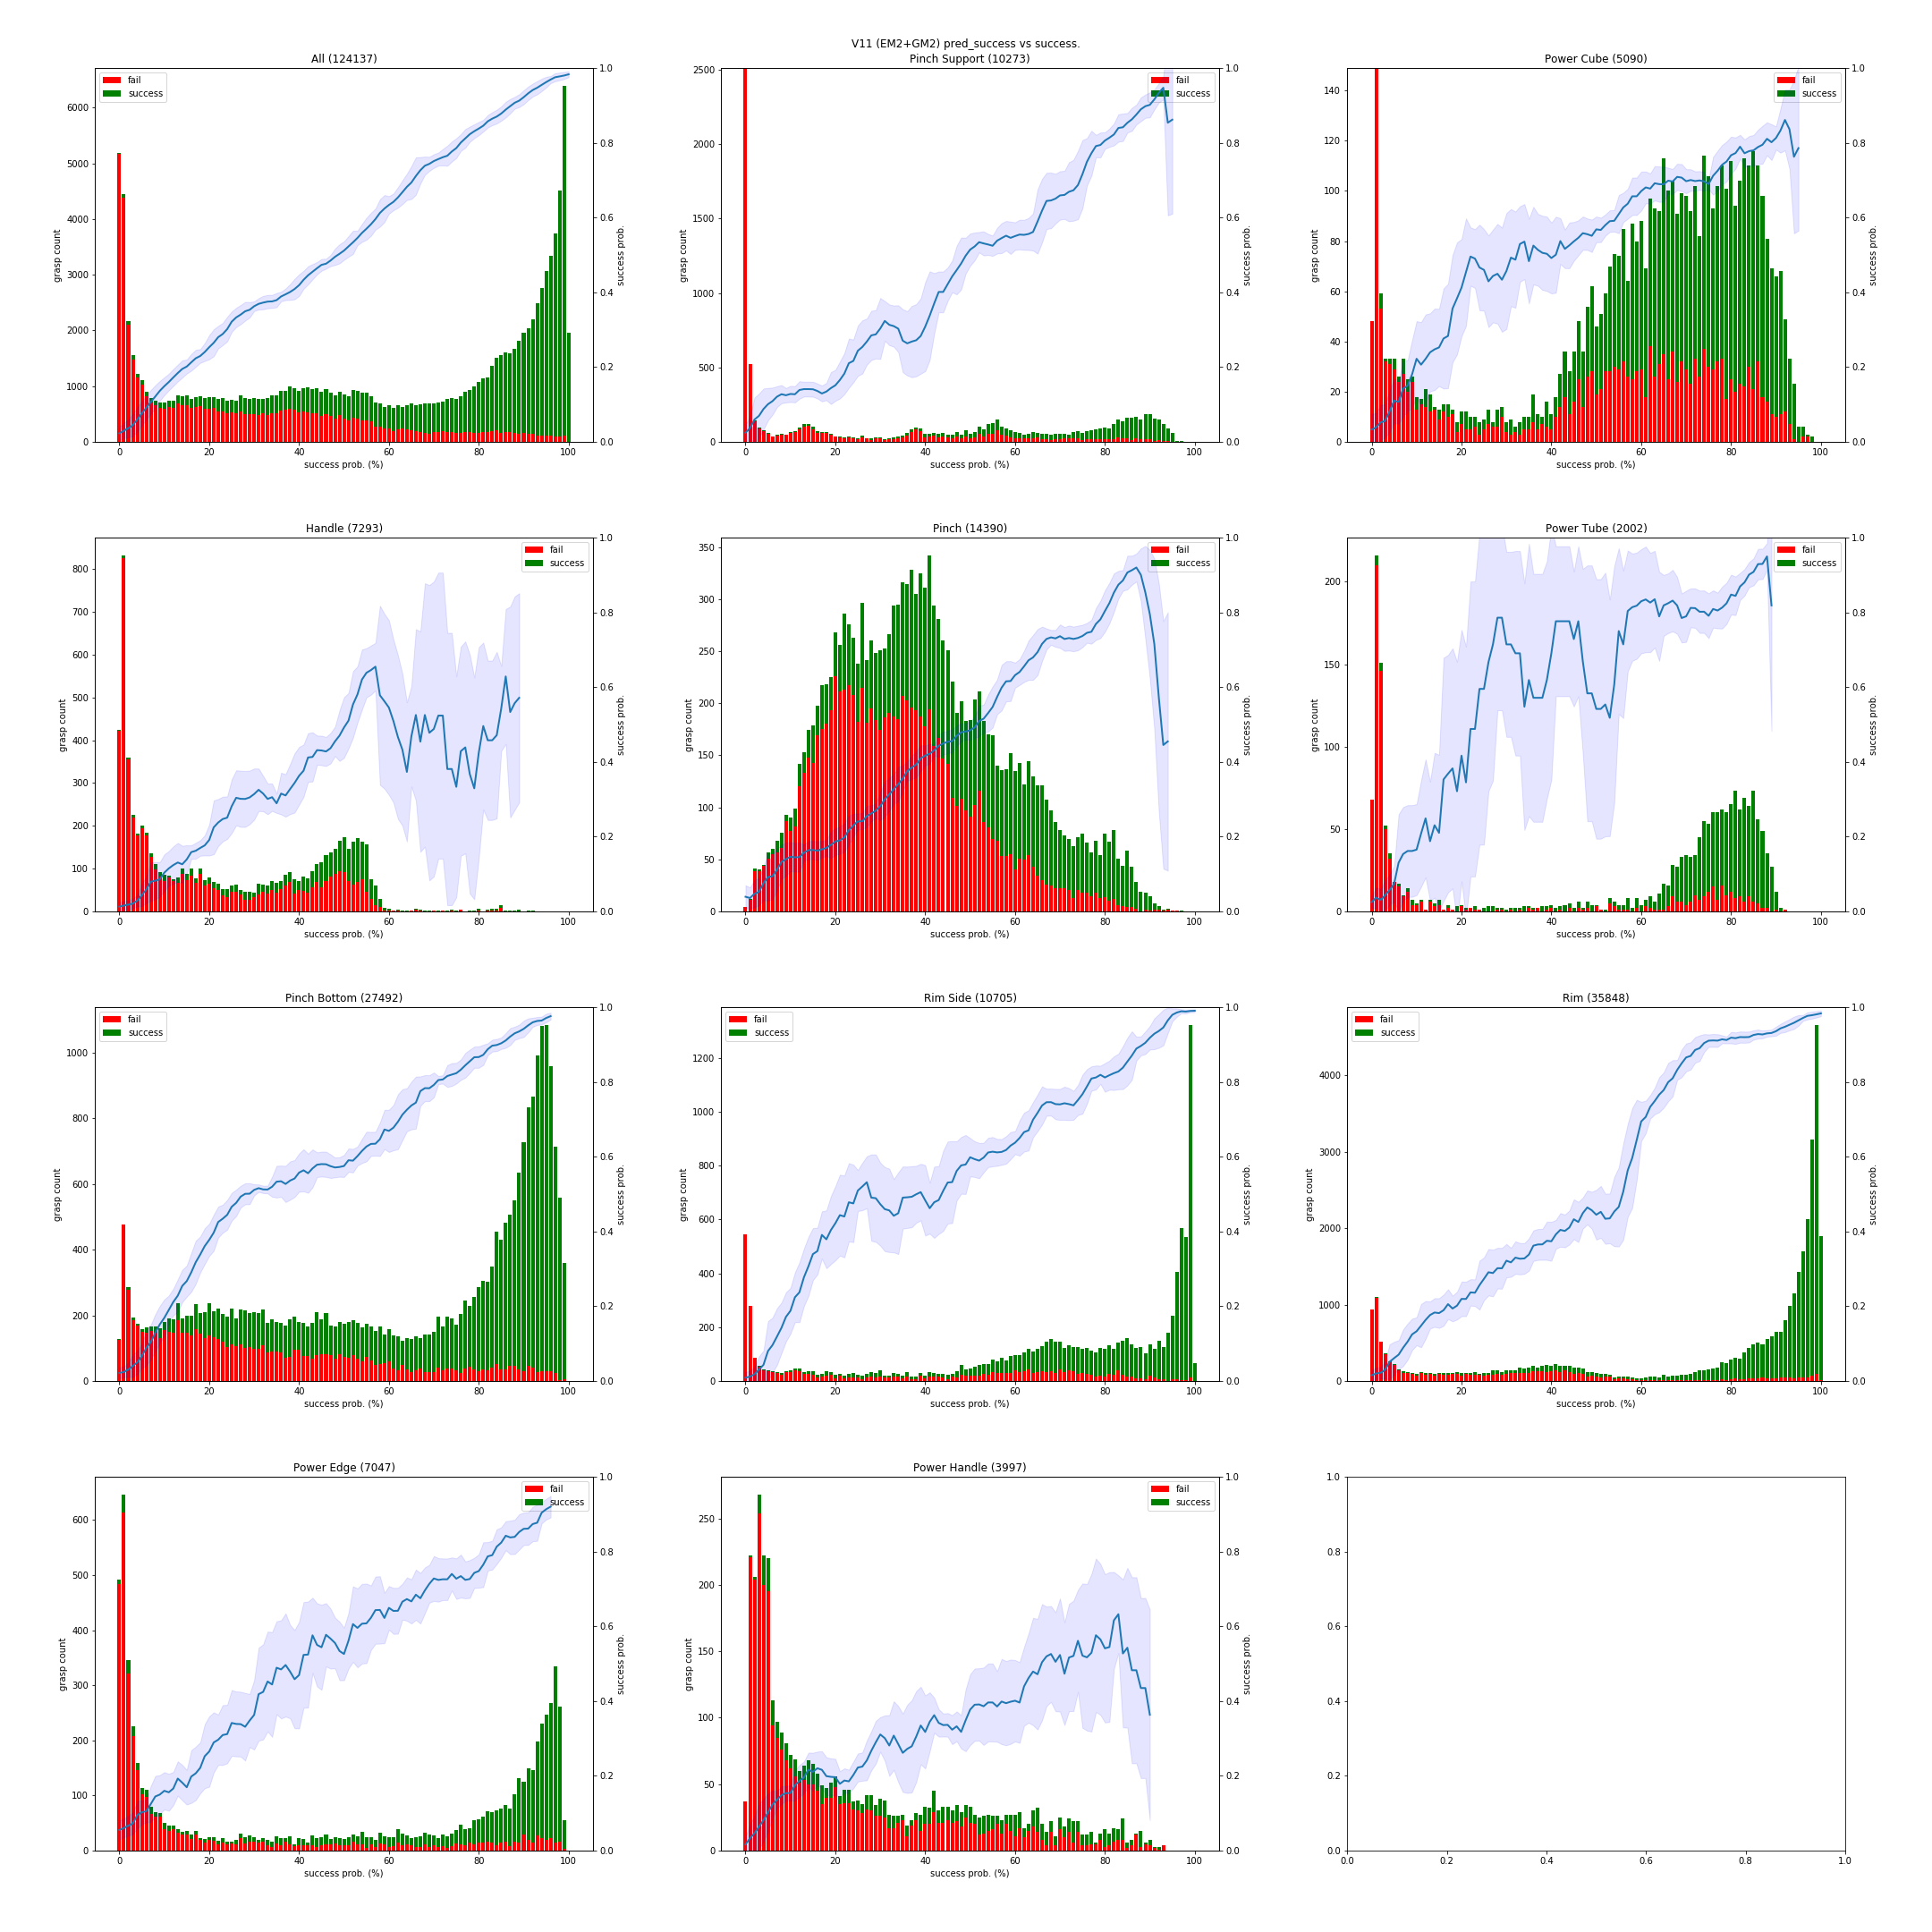
\includegraphics[width=0.8\columnwidth]{images/post-analysis/[4] V11_pred_success_vs_success.png}
\caption{Predicted success probability vs actual success probability for V11. The red bars indicate failures, and green bars show successes. The grasps are ordered along the horizontal axis by predicted success probabilities by EM3. The blue line shows the (actual) average success rate of grasps in every bin, while the vertical length of the shaded blue region around each point on the line correlates with the standard deviation of the success rates in nearby bins. Note that when data is missing from the graph, such as the Handle and Power Tube grasps, the noisiness of the success rate estimates increase significantly.}
\label{fig:calibrate}
\end{figure}


\subsection{Why is a combined architecture improving the performance?}
\noindent

V11, which combines the generative model GM2 with the evaluative model EM3, yields a substantial improvement over GM2's ranking, improving GM2's simulation top-grasp success rate from 79.05\% to 90.49\%, and real-world performance from 81.6\% to 87.8\%.Two main factors could contribute to this result. First, EM3 could be assigning high predicted success probabilities of grasp types that are generally successful, and low probabilities to those grasp types that fail often. Effectively, this would mean that a ranking based on EM3's assigned probabilities would favour grasp types that are generally successful over others. Second, within each grasp type, EM3 may be learning which grasps are more likely to be successful according to the hand position, orientation and finger configuration. The second one is more interesting. It implicates that given the visual perception of the object, the network would have to learn which grasp configurations are more likely to be successful, rather than simply picking them based on their types. Let us investigate which factors are at play.

\subsubsection{How does an evaluative model rank grasp types?}
\noindent


\begin{figure}
\centering 
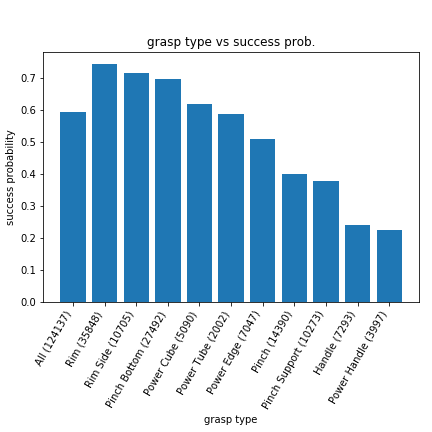
\includegraphics[width=0.6\columnwidth]{images/post-analysis/[2] Grasp_type_vs_success_prob.png}
\caption{Grasp type vs. success probability.}
\label{fig:post2}
\end{figure}

Not all grasps are created equal. On average, some grasp types are more successful than others. We found that grasp types where all five fingers have contact with the object, such as Rim, Rim Side, or Power Cube are generally more successful than the ones where only 2-3 fingers touch the object, e.g. Pinch and Handle variations. Figure~\ref{fig:post2} compares the average grasp success rates in the DS2-Te (GM2 Test) dataset, which shows this. We think this is due to the increased tolerance for error when more contacts are involved, and is consistent with the dynamics of humans grasping objects. 

Figure~\ref{fig:post6} compares 3 different rankings (random, V2, V11), and plots the distribution of grasp types for each position in all rankings. The random ranking which are based on randomly assigned success probabilities, predictably, uniformly places all grasps at all positions, regardless of their type. V2, which is based on the grasp success likelihoods generated by GM2, favours successful grasp types such as Rim variations over unsuccessful ones such as Handle grasps. V11, based on the evaluative model EM3, acts similarly to V2. Interestingly, V2 and V11 both appear to be taking the grasp type into account, despite calculating the grasp success probabilities in entirely different ways.

\begin{figure}
\centering
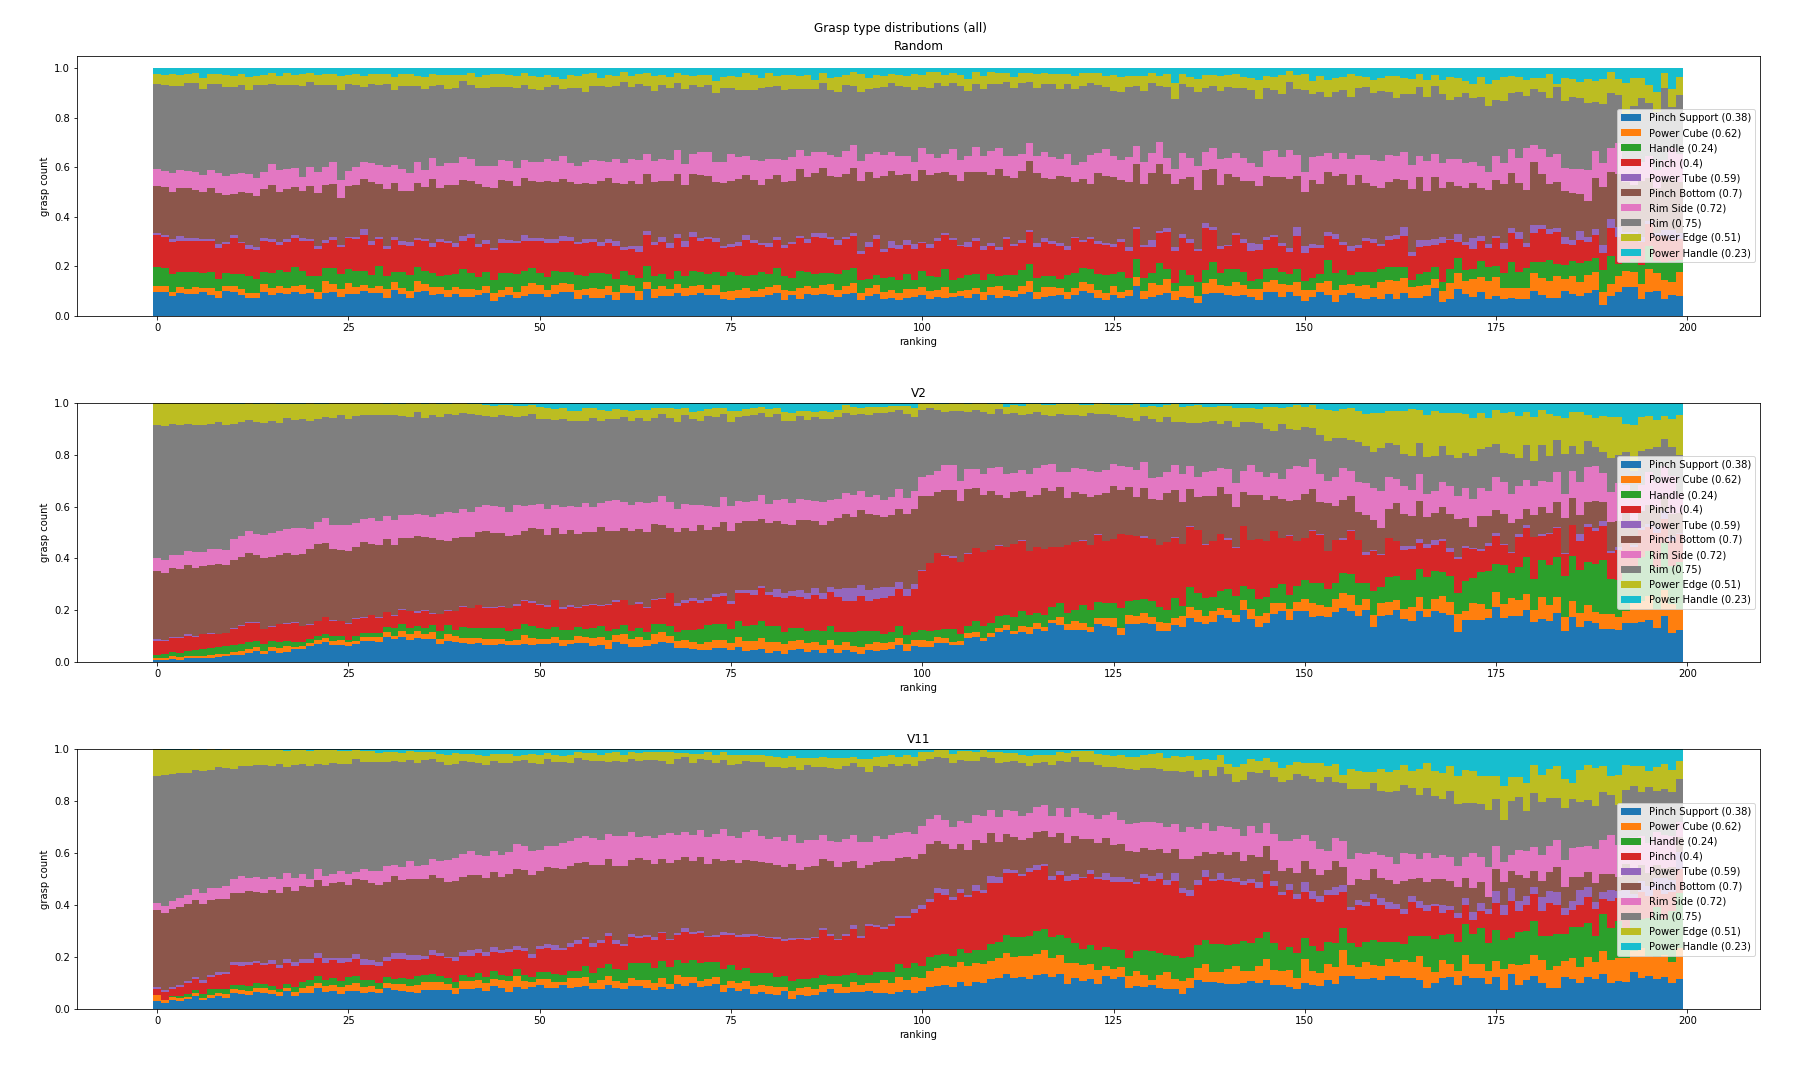
\includegraphics[width=0.8\columnwidth]{images/post-analysis/[6] Grasp_type_distributions_all.png}
\caption{Comparison of grasp type distributions per ranking of random ranking,V2 and V11.}
\label{fig:post6}
\end{figure}

%\begin{figure}
%\centering
%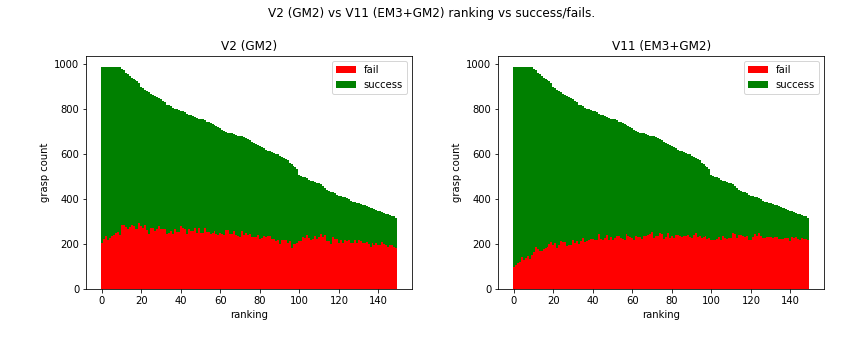
\includegraphics[width=0.8\columnwidth]{images/post-analysis/[3] V2_vs_V11_ranking_vs_success_fail.png}
%\caption{Comparison of successful (green) and unsuccessful (red) grasps per ranking for V2 and V11.}
%\label{fig:post3}
%\end{figure}

\subsubsection{Does EM3 rank grasps within a grasp type?}
\noindent

The second question we asked was whether EM3 is learning to rank grasps in each grasp type according to the visual input. 

\begin{figure}
\centering
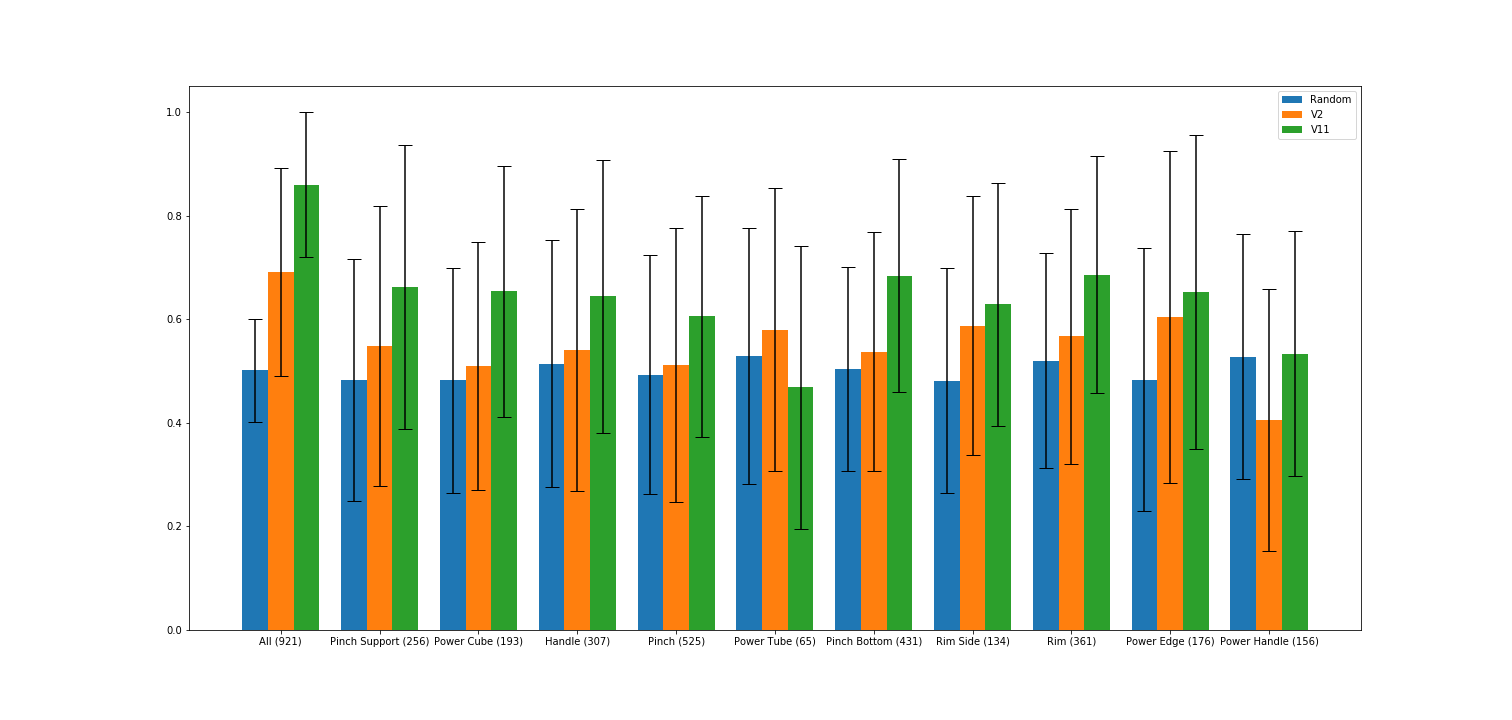
\includegraphics[width=0.999\columnwidth]{images/post-analysis/[5] Ranking_quality_mean_AUC.png}
\caption{Grasp ranking quality comparison of random ranking, V2 and V11.}
\label{fig:post5}
\end{figure}

\begin{figure}
\centering
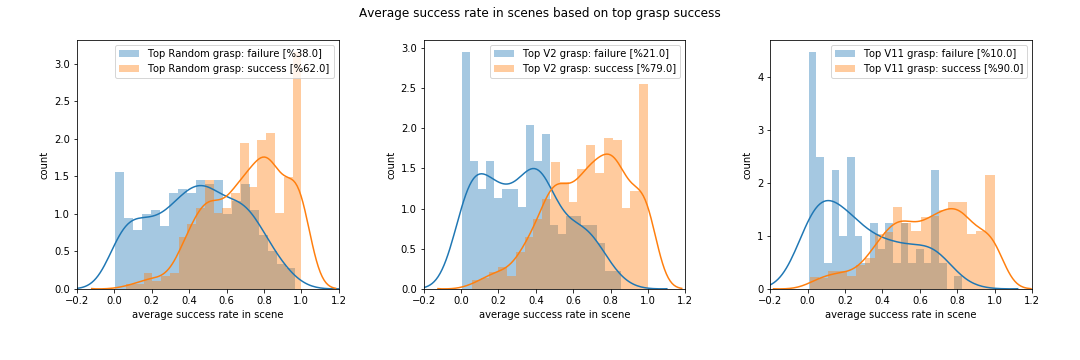
\includegraphics[width=0.8\columnwidth]{images/post-analysis/[7] Average_success_rate_in_scenes_based_on_top_grasp_success.png}
\caption{Average success rate in scenes vs top grasp success.}
\label{fig:post7}
\end{figure}

\begin{figure}
\centering
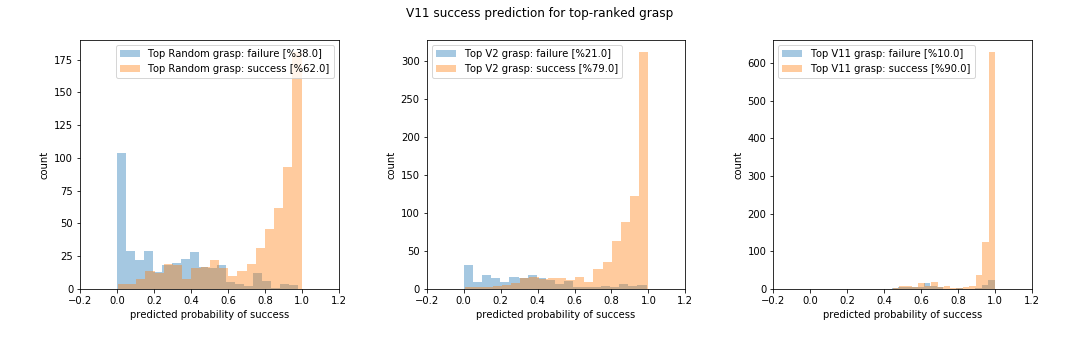
\includegraphics[width=0.8\columnwidth]{images/post-analysis/[8] V11_success_prediction_for_top-ranked_grasp.png}
\caption{Histogram of success rate of a top-ranked grasp vs its probability of success as estimated by V11.}
\label{fig:post8}
\end{figure}

\begin{figure}
\centering
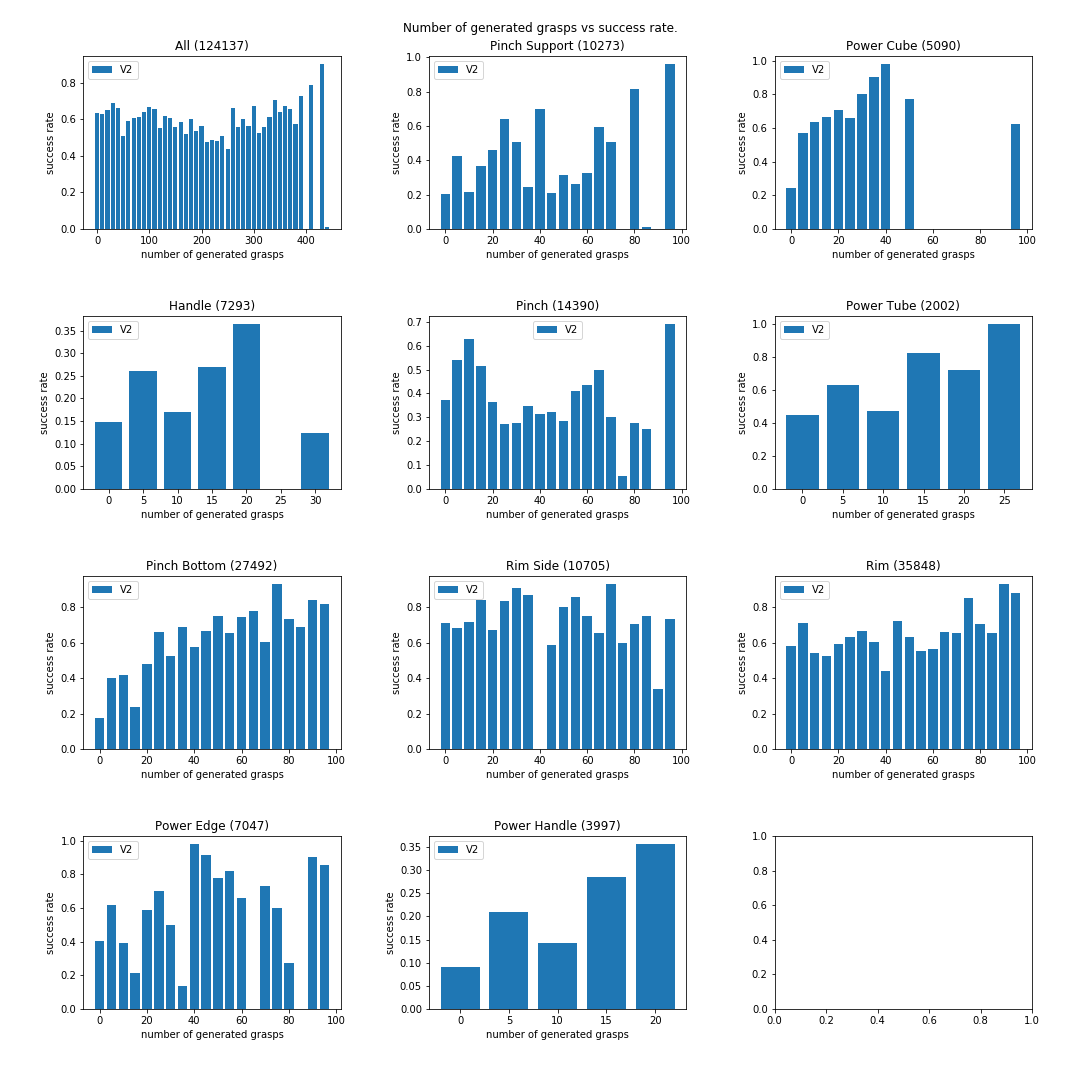
\includegraphics[width=0.8\columnwidth]{images/post-analysis/[10] number_of_generated_grasps_vs_success_rate.png}
\caption{Correlation of success rate with number of generated grasps per scene per grasp type.}
\label{fig:post10}
\end{figure}

\begin{figure}
\centering
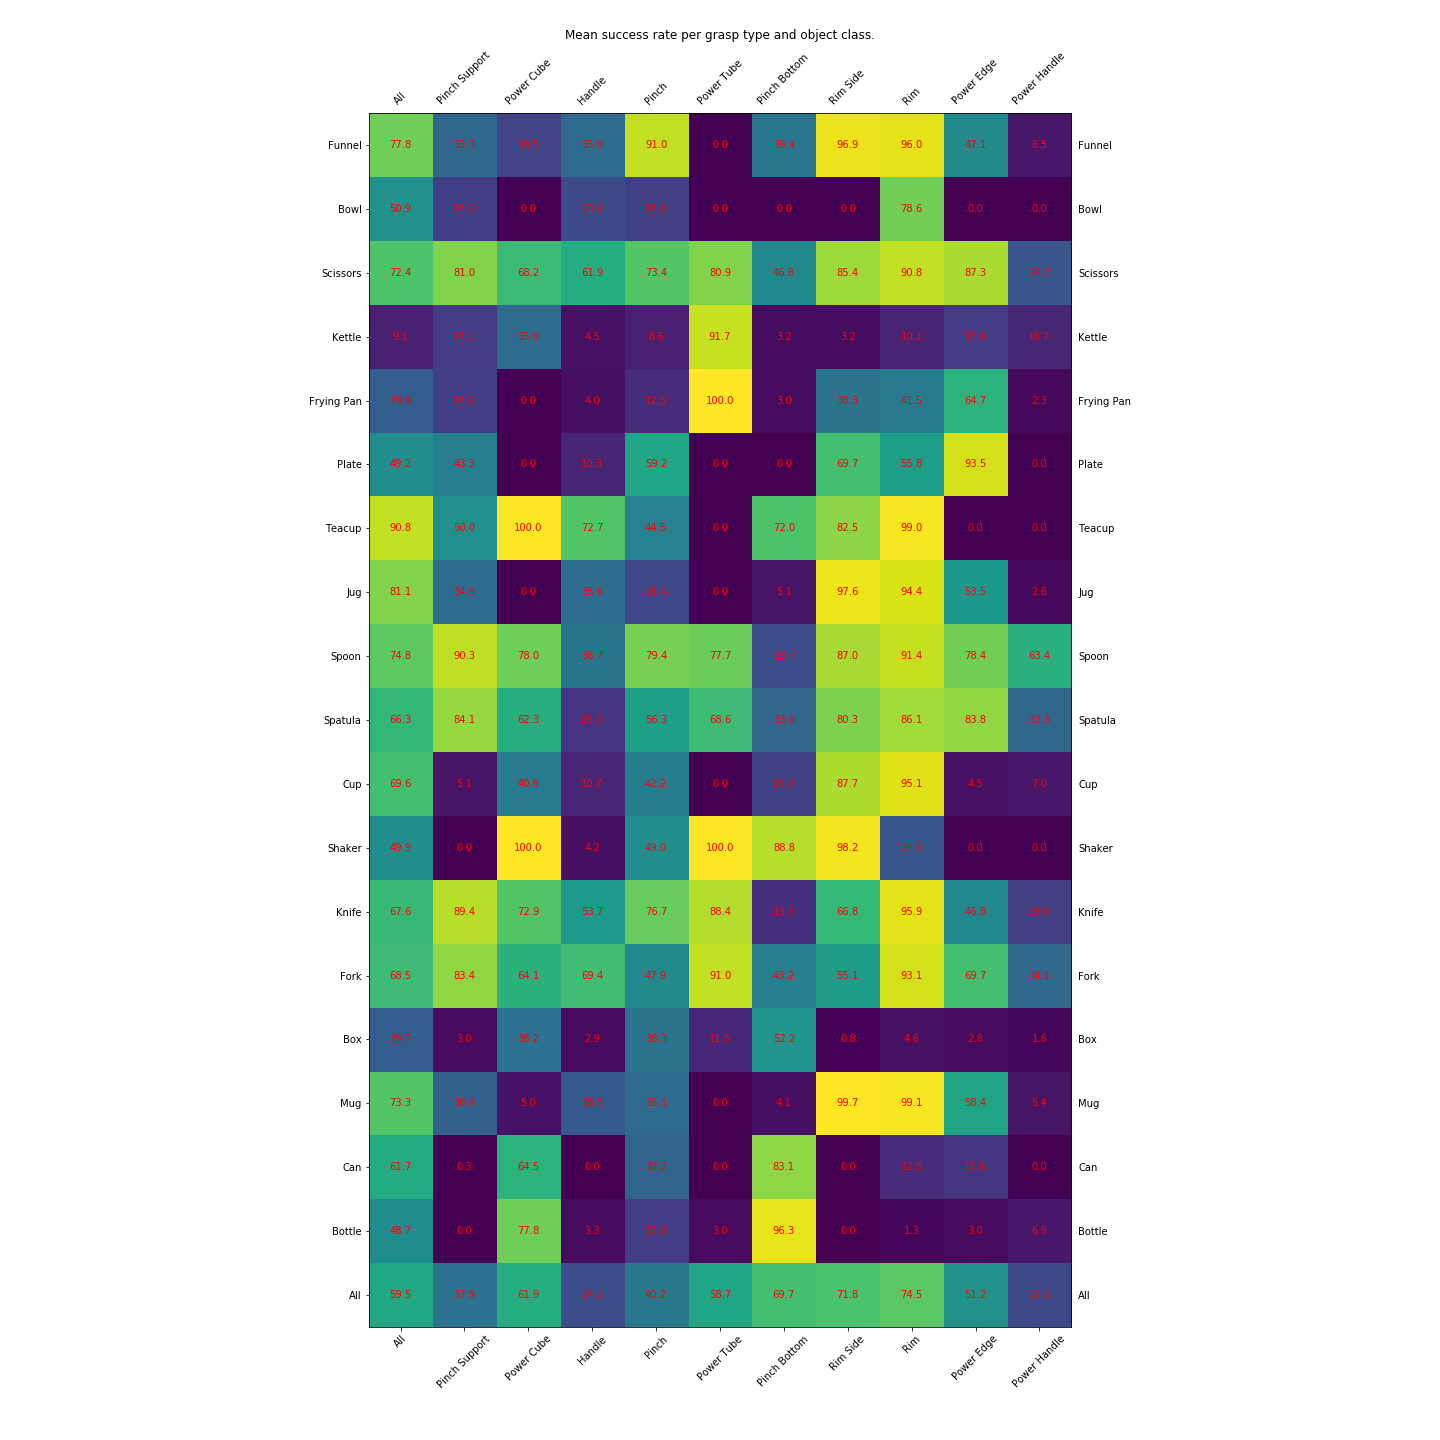
\includegraphics[width=0.8\columnwidth]{images/post-analysis/[12] mean_success_rate_per_grasp_type_and_object_class.png}
\caption{Mean success rate per grasp type and object class.}
\label{fig:post12}
\end{figure}

\begin{figure}
\centering
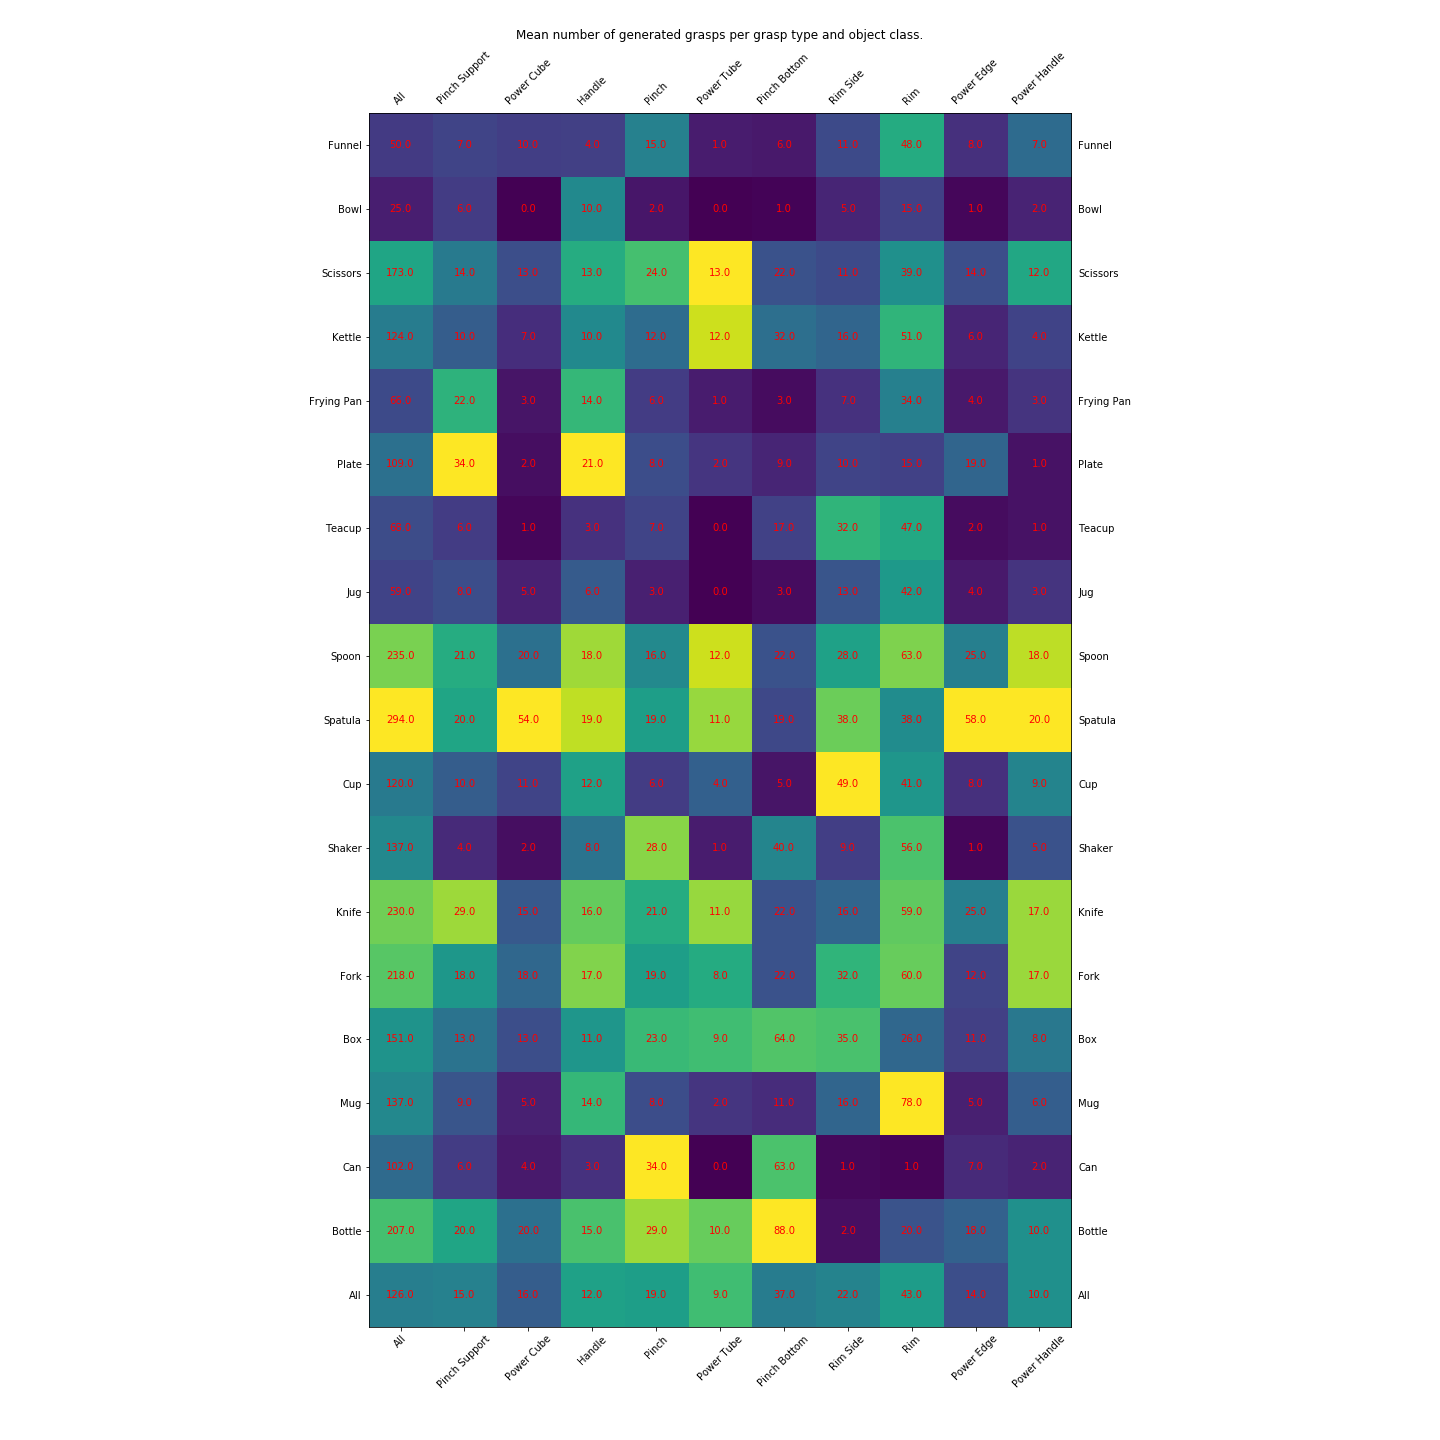
\includegraphics[width=0.8\columnwidth]{images/post-analysis/[13] mean_number_of_generated_grasps_per_grasp_type_and_object_class.png}
\caption{Mean number of generated grasps per grasp type and object class.}
\label{fig:post13}
\end{figure}


%We compared the EM and GM rankings (Figure~\ref{fig:successvsranking}). The x-axis shows the ranking. The y-axis shows the average actual success rate over all scenes (1,241 test, 7,311 training). When ranked by the EM, the grasp success probability falls nearly monotonically, as is desirable. On the other hand, the likelihood-based ranking of GM results in many good grasps being low-ranked. We also wish to know whether the grasps recommended by the EM and the GM have different grasp success rates. The success rates of the top-ranked grasps are 71.59\% (GM) and  84.2\% (EM).

%A pure generative model architecture (GM) and the generative-evaluative architecture (GEA) were evaluated using a paired trials methodology. Each was presented with the same object-pose combinations. Each architecture generated a ranked list of grasps, and the highest ranked grasp was executed. The highest-ranked grasp based on the predicted success probability of the network is performed on each scene. A grasp was deemed successful if, when lifted for five seconds, the object then remained stable in the hand for a further five seconds before being automatically released. The success rate for GM was 57.1\% and for GEA it was 77.6\%. The successes and failures for each method were recorded and are summarised in Table~\ref{tab:robot-results}. A two-tailed McNemar test, for the difference between success rates for paired comparison data, was performed and the difference between the two algorithms has a $p$-value of 0.0442, and so is statistically significant. A selection of grasps where the two methods performed differently are shown in Figure~\ref{fig:successfail}.

% OLD TABLE
%\begin{table}
%\begin{center}
%\caption{Results of the real robot paired comparison trial.}
%\begin{tabular}{|c|c|c|c|}  \hline 
%          &                & \multicolumn{2}{ c |}{ GM} \\ \hline
%          &                & \# succs & \# fails  \\  \hline
 %GEA  & \# succs &  23 &  15  \\
 %         & \# fails    &  5   &   6   \\ \hline
%\end{tabular}
%\end{center}
%\label{tab:robot-results}
%\end{table}

%Training parameters for network. Training of example grasps for learning from demonstration. Creation of real test data set. Paired comparisons methodology with vanilla LFD algorithm (pose + object + camera view).
%
%The actual grasping tests have been performed on the real robot. 